\problemname{Crooked Dealing}

This week you started a flashy new job in Leeds as a poker dealer. Your task
will be to hand out the cards for games. The base pay is not particularly good,
but you found out that you can earn a lot from tips if you deal the cards well.

The most generous customers prefer that their opponents at the table don't
receive any pairs of cards with the same number; so to keep them happy you will
make sure this never happens.

You already know the numbers on every card in the pile , and the number of
cards any player must have in their hand. Find how many hands you can make at
once without introducing a pair.

\begin{figure}[h!]
  \centering
  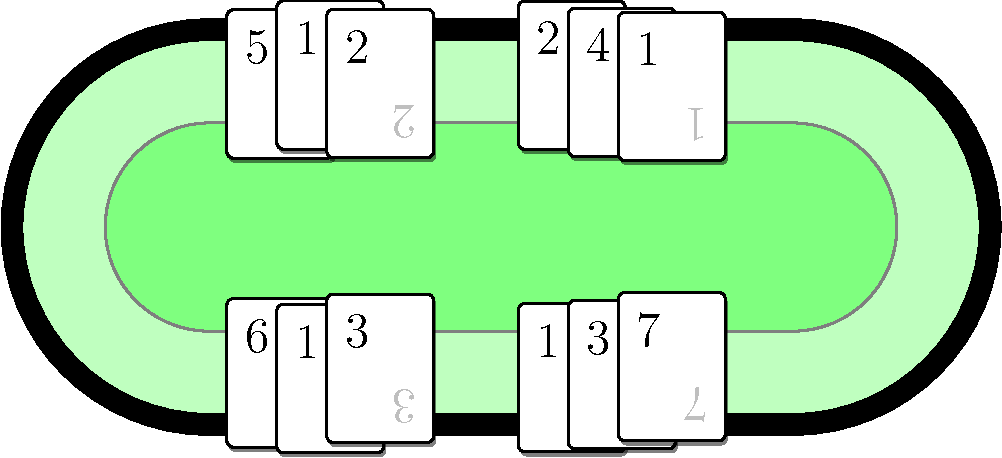
\includegraphics[width=0.9\textwidth]{sample}
  \caption{Illustration of a solution to Sample Input 2.}
  \label{fig:crookeddealing}
\end{figure}

\section*{Input}
The input consists of:
  \begin{itemize}
    \item A line with two integers $n$ and $h$ ($1 \le h \le n \le 10^6$), the
          number of cards in the pile, and the number of cards in a hand.
    \item A line with $n$ integers $v_1, \ldots, v_n$ ($1 \le v_i \le 10^6$
          for all $i$), the numbers on the cards in no particular order.
  \end{itemize}

\section*{Output}
  If it is not possible to make any hands at all without introducing a pair,
  output \texttt{impossible}.

  Otherwise, output $k$ lines (where $k$ is the maximum possible number of
  players) each containing $h$ numbers from the input. You may not use any
  number any more times than it appears in $v$.

  If there are multiple answers with a maximum value of $k$, you may output any
  one of them.
